% !TEX encoding = UTF-8 Unicode
% !TEX TS-program = xelatex 
\begin{QUESTIONS}
    \begin{QUESTION}
        \begin{ExamInfo}{105}{學測}{單選}{1}
        \end{ExamInfo}
        \begin{ExamAnsRateInfo}{67}{97}{77}{27}
        \end{ExamAnsRateInfo}
        \begin{QBODY}
			設$f(x)$為二次實係數多項式,已知$f(x)$在$x=2$時有最小值1且$f(3)=3$。請問$f(1)$之值為下列哪一選項?
			\begin{QOPS}
				\QOP 5	
				\QOP 2	
				\QOP 3
				\QOP 4	
				\QOP 條件不足,無法確定
			\end{QOPS}
        \end{QBODY}
        \begin{QFROMS}
        \end{QFROMS}
        \begin{QTAGS}\QTAG{B1C2多項式函數}\end{QTAGS}
        \begin{QANS}
            (3)
        \end{QANS}
        \begin{QSOLLIST}
        \end{QSOLLIST}
        \begin{QEMPTYSPACE}
        \end{QEMPTYSPACE}
    \end{QUESTION}
    \begin{QUESTION}
        \begin{ExamInfo}{105}{學測}{單選}{2}
        \end{ExamInfo}
        \begin{ExamAnsRateInfo}{53}{89}{58}{12}
        \end{ExamAnsRateInfo}
        \begin{QBODY}
			請問$\sin 73{}^\circ $、$\sin 146{}^\circ $、$\sin 219{}^\circ $、$\sin 292{}^\circ $、$\sin 365{}^\circ $這五個數值的中位數是哪一個?
			\begin{QOPS}
				\QOP $\sin 73{}^\circ $	
				\QOP $\sin 146{}^\circ $	
				\QOP $\sin 219{}^\circ $
				\QOP $\sin 292{}^\circ $	
				\QOP $\sin 365{}^\circ $
			\end{QOPS}
        \end{QBODY}
        \begin{QFROMS}
        \end{QFROMS}
        \begin{QTAGS}\QTAG{B3C1三角}\end{QTAGS}
        \begin{QANS}
            (5)
        \end{QANS}
        \begin{QSOLLIST}
        \end{QSOLLIST}
        \begin{QEMPTYSPACE}
        \end{QEMPTYSPACE}
    \end{QUESTION}
    \begin{QUESTION}
        \begin{ExamInfo}{105}{學測}{單選}{3}
        \end{ExamInfo}
        \begin{ExamAnsRateInfo}{54}{77}{53}{32}
        \end{ExamAnsRateInfo}
        \begin{QBODY}
			坐標平面上兩圖形${{\Gamma }_{1}},{{\Gamma }_{2}}$的方程式分別為:${{\Gamma }_{1}}:{{(x+1)}^{2}}+{{y}^{2}}=1$、${{\Gamma }_{2}}:{{(x+y)}^{2}}=1$。請問${{\Gamma }_{1}},{{\Gamma }_{2}}$共有幾個交點?
			\begin{QOPS}
				\QOP 1個	
				\QOP 2個	
				\QOP 3個	
				\QOP 4個	
				\QOP 0個
			\end{QOPS}
        \end{QBODY}
        \begin{QFROMS}
        \end{QFROMS}
        \begin{QTAGS}\QTAG{B4C4二次曲線}\end{QTAGS}
        \begin{QANS}
            (2)
        \end{QANS}
        \begin{QSOLLIST}
        \end{QSOLLIST}
        \begin{QEMPTYSPACE}
        \end{QEMPTYSPACE}
    \end{QUESTION}
    \begin{QUESTION}
        \begin{ExamInfo}{105}{學測}{單選}{4}
        \end{ExamInfo}
        \begin{ExamAnsRateInfo}{54}{91}{55}{16}
        \end{ExamAnsRateInfo}
        \begin{QBODY}
			放射性物質的半衰期$T$定義為每經過時間$T$,該物質的質量會衰退成原來的一半。鉛製容器中有兩種放射性物質$A$、$B$,開始紀錄時容器中物質$A$的質量為物質$B$的兩倍,而120小時後兩種物質的質量相同。已知物質$A$的半衰期為7.5小時,請問物質$B$的半衰期為幾小時?
			\begin{QOPS}
				\QOP 8小時	
				\QOP 10小時	
				\QOP 12小時	
				\QOP 15小時	
				\QOP 20小時
			\end{QOPS}
        \end{QBODY}
        \begin{QFROMS}
        \end{QFROMS}
        \begin{QTAGS}\QTAG{B1C3指對數函數}\end{QTAGS}
        \begin{QANS}
            (1)
        \end{QANS}
        \begin{QSOLLIST}
        \end{QSOLLIST}
        \begin{QEMPTYSPACE}
        \end{QEMPTYSPACE}
    \end{QUESTION}
    \begin{QUESTION}
        \begin{ExamInfo}{105}{學測}{單選}{5}
        \end{ExamInfo}
        \begin{ExamAnsRateInfo}{52}{86}{49}{21}
        \end{ExamAnsRateInfo}
        \begin{QBODY}
			坐標空間中一質點自點$P(1,1,1)$沿著方向$\lvec{a}=(1,2,2)$等速直線前進,經過5秒後剛好到達平面$x-y+3z=28$上,立即轉向沿著方向$\lvec{b}=(-2,2,-1)$依同樣的速率等速直線前進。請問再經過幾秒此質點會剛好到達平面$x=2$上?
			\begin{QOPS}
				\QOP 1秒
				\QOP 2秒
				\QOP 3秒
				\QOP 4秒
				\QOP 永遠不會到達
			\end{QOPS}
        \end{QBODY}
        \begin{QFROMS}
        \end{QFROMS}
        \begin{QTAGS}\QTAG{B4C1空間向量}\end{QTAGS}
        \begin{QANS}
            (2)
        \end{QANS}
        \begin{QSOLLIST}
        \end{QSOLLIST}
        \begin{QEMPTYSPACE}
        \end{QEMPTYSPACE}
    \end{QUESTION}
    \begin{QUESTION}
        \begin{ExamInfo}{105}{學測}{單選}{6}
        \end{ExamInfo}
        \begin{ExamAnsRateInfo}{28}{53}{22}{9}
        \end{ExamAnsRateInfo}
        \begin{QBODY}
			設$\left\langle {{a}_{n}} \right\rangle $為一等比數列。已知前十項的和為$\sum\limits_{k=1}^{10}{{{a}_{k}}}=80$,前五個奇數項的和為${{a}_{1}}+{{a}_{3}}+{{a}_{5}}+{{a}_{7}}+{{a}_{9}}=120$,請選出首項${{a}_{1}}$的正確範圍。
			\begin{QOPS}
				\QOP ${{a}_{1}}<80$
				\QOP $80\le {{a}_{1}}<90$
				\QOP $90\le {{a}_{1}}<100$
				\QOP $100\le {{a}_{1}}<110$
				\QOP $110\le {{a}_{1}}$
			\end{QOPS}
        \end{QBODY}
        \begin{QFROMS}
        \end{QFROMS}
        \begin{QTAGS}\QTAG{B2C1數列級數}\end{QTAGS}
        \begin{QANS}
            (4)
        \end{QANS}
        \begin{QSOLLIST}
        \end{QSOLLIST}
        \begin{QEMPTYSPACE}
        \end{QEMPTYSPACE}
    \end{QUESTION}
\end{QUESTIONS}
\begin{QUESTIONS}
    \begin{QUESTION}
        \begin{ExamInfo}{105}{學測}{多選}{7}
        \end{ExamInfo}
        \begin{ExamAnsRateInfo}{54}{81}{52}{29}
        \end{ExamAnsRateInfo}
        \begin{QBODY}
			下列各方程式中,請選出有實數解的選項。
			\begin{QOPS}
				\QOP $\left| x \right|+\left| x-5 \right|=1$
				\QOP $\left| x \right|+\left| x-5 \right|=6$
				\QOP $\left| x \right|-\left| x-5 \right|=1$
				\QOP $\left| x \right|-\left| x-5 \right|=6$
				\QOP $\left| x \right|-\left| x-5 \right|=-1$
			\end{QOPS}
        \end{QBODY}
        \begin{QFROMS}
        \end{QFROMS}
        \begin{QTAGS}\QTAG{B1C1數與式}\end{QTAGS}
        \begin{QANS}
            (2)(3)(5)
        \end{QANS}
        \begin{QSOLLIST}
        \end{QSOLLIST}
        \begin{QEMPTYSPACE}
        \end{QEMPTYSPACE}
    \end{QUESTION}
    \begin{QUESTION}
        \begin{ExamInfo}{105}{學測}{多選}{8}
        \end{ExamInfo}
        \begin{ExamAnsRateInfo}{59}{77}{60}{40}
        \end{ExamAnsRateInfo}
        \begin{QBODY}
			下面是甲、乙兩個商場的奇異果以及蘋果不同包裝的價格表,例如:甲商場奇異果價格「35元/一袋2顆」表示每一袋有2顆奇異果,價格35元。
			甲商場售價
			\begin{tabular}{|c|c|c|c|c|}
			\hline
				奇異果價格	& 20元/一袋1顆	& 35元/一袋2顆	& 80元/一袋5顆	& 100元/一袋6顆 \\\hline
				蘋果價格	& 45元/一袋1顆	& 130元/一袋3顆	& 260元/一袋6顆	& 340元/一袋8顆 \\\hline
			\end{tabular}
			乙商場售價
			\begin{tabular}{|c|c|c|c|c|}
			\hline			
			奇異果價格  & 18元/一袋1顆	& 50元/一袋3顆	& 65元/一袋4顆	& 95元/一袋6顆 \\\hline
			蘋果價格	& 50元/一袋1顆	& 190元/一袋4顆	& 280元/一袋6顆	& 420元/一袋10顆\\\hline
			\end{tabular}
			依據上述數據,請選出正確的選項。
			\begin{QOPS}
				\QOP 在甲商場買一袋3顆裝的蘋果所需金額低於買三袋1顆裝的蘋果
				\QOP 乙商場的奇異果售價,一袋裝越多顆者,其每顆單價越低
				\QOP 若只想買奇異果,則在甲商場花500元最多可以買到30顆奇異果
				\QOP 如果要買12顆奇異果和4顆蘋果,在甲商場所需最少金額低於在乙商場所需最少金額
				\QOP 無論要買多少顆蘋果,在甲商場所需最少金額都低於在乙商場所需最少金額
			\end{QOPS}
        \end{QBODY}
        \begin{QFROMS}
        \end{QFROMS}
        \begin{QTAGS}\QTAG{綜合}\end{QTAGS}
        \begin{QANS}
            (1)(2)(4)
        \end{QANS}
        \begin{QSOLLIST}
        \end{QSOLLIST}
        \begin{QEMPTYSPACE}
        \end{QEMPTYSPACE}
    \end{QUESTION}
    \begin{QUESTION}
        \begin{ExamInfo}{105}{學測}{多選}{9}
        \end{ExamInfo}
        \begin{ExamAnsRateInfo}{46}{77}{40}{21}
        \end{ExamAnsRateInfo}
        \begin{QBODY}
		下列各直線中,請選出和$z$軸互為歪斜線的選項。
			\begin{QOPS}
				\QOP ${{L}_{1}}:\text{ }\left\{ \begin{aligned}
				  & x=0 \\ 
				 & z=0 \\ 
				\end{aligned} \right.$	
                \QOP ${{L}_{\text{2}}}:\text{ }\left\{ \begin{aligned}
				  & y=0 \\ 
				 & x+z=1 \\ 
				\end{aligned} \right.$	
                \QOP ${{L}_{3}}:\text{ }\left\{ \begin{aligned}
				  & z=0 \\ 
				 & x+y=1 \\ 
				\end{aligned} \right.$
				\QOP ${{L}_{4}}:\left\{ \begin{aligned}
				  & x=1 \\ 
				 & y=1 \\ 
				\end{aligned} \right.$	
                \QOP ${{L}_{5}}:\left\{ \begin{aligned}
				  & y=1 \\ 
				 & z=1 \\ 
				\end{aligned} \right. $
			\end{QOPS}
        \end{QBODY}
        \begin{QFROMS}
        \end{QFROMS}
        \begin{QTAGS}\QTAG{B4C1空間向量}\end{QTAGS}
        \begin{QANS}
            (3)(5)
        \end{QANS}
        \begin{QSOLLIST}
        \end{QSOLLIST}
        \begin{QEMPTYSPACE}
        \end{QEMPTYSPACE}
    \end{QUESTION}
    \begin{QUESTION}
        \begin{ExamInfo}{105}{學測}{多選}{10}
        \end{ExamInfo}
        \begin{ExamAnsRateInfo}{34}{59}{28}{15}
        \end{ExamAnsRateInfo}
        \begin{QBODY}
			設$a$、$b$、$c$皆為正整數,考慮多項式$f(x)={{x}^{4}}+a{{x}^{3}}+b{{x}^{2}}+cx+2$。請選出正確的選項。
			\begin{QOPS}
				\QOP $f(x)=0$無正根
				\QOP $f(x)=0$一定有實根
				\QOP $f(x)=0$一定有虛根
				\QOP $f(1)+f(-1)$的值是偶數
				\QOP 若$a+c>b+3$,則$f(x)=0$有一根介於$-1$與0之間
			\end{QOPS}
        \end{QBODY}
        \begin{QFROMS}
        \end{QFROMS}
        \begin{QTAGS}\QTAG{B1C2多項式函數}\end{QTAGS}
        \begin{QANS}
            (1)(4)(5)
        \end{QANS}
        \begin{QSOLLIST}
        \end{QSOLLIST}
        \begin{QEMPTYSPACE}
        \end{QEMPTYSPACE}
    \end{QUESTION}
    \begin{QUESTION}
        \begin{ExamInfo}{105}{學測}{多選}{11}
        \end{ExamInfo}
        \begin{ExamAnsRateInfo}{47}{67}{49}{25}
        \end{ExamAnsRateInfo}
        \begin{QBODY}
			一個41人的班級某次數學考試,每個人的成績都未超過59分。老師決定以下列方式調整成績:原始成績為$x$分的學生,新成績調整為$40{{\log }_{10}}(\FR{x+1}{10})+60$分(四捨五入到整數)。請選出正確的選項。
			\begin{QOPS}
				\QOP 若某人原始成績是9分,則新成績為60分
				\QOP 若某人原始成績超過20分,則其新成績超過70分
				\QOP 調整後全班成績的全距比原始成績的全距大
				\QOP 已知小文的原始成績恰等於全班原始成績的中位數,則小文的新成績仍然等於調整後全班成績的中位數
				\QOP 已知小美的原始成績恰等於全班原始成績的平均,則小美的新成績仍然等於調整後全班成績的平均(四捨五入到整數)
			\end{QOPS}
		\end{QBODY}
        \begin{QFROMS}
        \end{QFROMS}
        \begin{QTAGS}\QTAG{B2C4數據分析}\end{QTAGS}
        \begin{QANS}
            (1)(2)(4)
        \end{QANS}
        \begin{QSOLLIST}
        \end{QSOLLIST}
        \begin{QEMPTYSPACE}
        \end{QEMPTYSPACE}
    \end{QUESTION}
    \begin{QUESTION}
        \begin{ExamInfo}{105}{學測}{多選}{12}
        \end{ExamInfo}
        \begin{ExamAnsRateInfo}{30}{46}{27}{17}
        \end{ExamAnsRateInfo}
        \begin{QBODY}
			在$\Delta ABC$中,已知$\angle A=20{}^\circ $、$\overline{AB}=5$、$\overline{BC}=4$。請選出正確的選項。
			\begin{QOPS}
				\QOP 可以確定$\angle B$的餘弦值
				\QOP 可以確定$\angle C$的正弦值
				\QOP 可以確定$\Delta ABC$的面積
				\QOP 可以確定$\Delta ABC$的內切圓半徑
				\QOP 可以確定$\Delta ABC$的外接圓半徑
			\end{QOPS}
        \end{QBODY}
        \begin{QFROMS}
        \end{QFROMS}
        \begin{QTAGS}\QTAG{B3C1三角}\end{QTAGS}
        \begin{QANS}
            (2)(5)
        \end{QANS}
        \begin{QSOLLIST}
        \end{QSOLLIST}
        \begin{QEMPTYSPACE}
        \end{QEMPTYSPACE}
    \end{QUESTION}
    \begin{QUESTION}
        \begin{ExamInfo}{105}{學測}{多選}{13}
        \end{ExamInfo}
        \begin{ExamAnsRateInfo}{56}{77}{58}{33}
        \end{ExamAnsRateInfo}
        \begin{QBODY}
			甲、乙、丙、丁四位男生各騎一台機車約$A$、$B$、$C$、$D$四位女生一起出遊,他們約定讓四位女生依照$A$、$B$、$C$、$D$的順序抽鑰匙來決定搭乘哪位男生的機車。其中除了$B$認得甲的機車鑰匙,並且絕對不會選取之外,每個女生選取這些鑰匙的機會都均等。請選出正確的選項。
			\begin{QOPS}
				\QOP $A$抽到甲的鑰匙的機率大於$C$抽到甲的鑰匙的機率
				\QOP $C$抽到甲的鑰匙的機率大於$D$抽到甲的鑰匙的機率
				\QOP $A$抽到乙的鑰匙的機率大於$B$抽到乙的鑰匙的機率
				\QOP $B$抽到丙的鑰匙的機率大於$C$抽到丙的鑰匙的機率
				\QOP $C$抽到甲的鑰匙的機率大於$C$抽到乙的鑰匙的機率
			\end{QOPS}
        \end{QBODY}
        \begin{QFROMS}
        \end{QFROMS}
        \begin{QTAGS}\QTAG{B2C3機率}\end{QTAGS}
        \begin{QANS}
            (4)(5)
        \end{QANS}
        \begin{QSOLLIST}
        \end{QSOLLIST}
        \begin{QEMPTYSPACE}
        \end{QEMPTYSPACE}
    \end{QUESTION}
\end{QUESTIONS}
\begin{QUESTIONS}
    \begin{QUESTION}
        \begin{ExamInfo}{105}{學測}{填充}{A}
        \end{ExamInfo}
        \begin{ExamAnsRateInfo}{22}{47}{16}{3}
        \end{ExamAnsRateInfo}
        \begin{QBODY}
			考慮每個元(或稱元素)只能是0或1的$2\times 3$階矩陣,且它的第一列與第二列不相同且各列的元素不能全為零,這樣的矩陣共有$\TCNBOX{\TCN\TCN}$ 個。
        \end{QBODY}
        \begin{QFROMS}
        \end{QFROMS}
        \begin{QTAGS}\QTAG{B4C3矩陣}\end{QTAGS}
        \begin{QANS}
            $42$
        \end{QANS}
        \begin{QSOLLIST}
        \end{QSOLLIST}
        \begin{QEMPTYSPACE}
        \end{QEMPTYSPACE}
    \end{QUESTION}
    \begin{QUESTION}
        \begin{ExamInfo}{105}{學測}{填充}{B}
        \end{ExamInfo}
        \begin{ExamAnsRateInfo}{22}{54}{11}{1}
        \end{ExamAnsRateInfo}
        \begin{QBODY}
			坐標平面上$O$為原點,設$\lvec{u}$$=(1,2)$、$\lvec{v}=(3,4)$。令$\Omega $為滿足$\lvec{OP}=x\lvec{u}+y\lvec{v}$的所有點$P$所形成的區域,其中$\FR{1}{2}\le x\le 1\ $、$-3\le y\le \FR{1}{2}$,則$\Omega $的面積為$\TCNBOX{\FR{\TCN}{\TCN}}$平方單位。(化成最簡分數)
        \end{QBODY}
        \begin{QFROMS}
        \end{QFROMS}
        \begin{QTAGS}\QTAG{B3C3平面向量}\end{QTAGS}
        \begin{QANS}
            $\dfrac{7}{2}$
        \end{QANS}
        \begin{QSOLLIST}
        \end{QSOLLIST}
        \begin{QEMPTYSPACE}
        \end{QEMPTYSPACE}
    \end{QUESTION}
    \begin{QUESTION}
        \begin{ExamInfo}{105}{學測}{填充}{C}
        \end{ExamInfo}
        \begin{ExamAnsRateInfo}{43}{85}{40}{4}
        \end{ExamAnsRateInfo}
        \begin{QBODY}
			從橢圓$\Gamma $的兩焦點分別作垂直於長軸的直線,交橢圓於四點。已知連此四點得一個邊長為2的正方形,則$\Gamma $的長軸長為$\TCNBOX{\TCN +\sqrt{\TCN}}$。
        \end{QBODY}
        \begin{QFROMS}
        \end{QFROMS}
        \begin{QTAGS}\QTAG{B4C4二次曲線}\end{QTAGS}
        \begin{QANS}
            $1+\sqrt{5}$
        \end{QANS}
        \begin{QSOLLIST}
        \end{QSOLLIST}
        \begin{QEMPTYSPACE}
        \end{QEMPTYSPACE}
    \end{QUESTION}
    \begin{QUESTION}
        \begin{ExamInfo}{105}{學測}{填充}{D}
        \end{ExamInfo}
        \begin{ExamAnsRateInfo}{51}{86}{56}{11}
        \end{ExamAnsRateInfo}
        \begin{QBODY}
		線性方程組$\left\{ \begin{aligned}
			 & x+2y+3z=0 \\ 
			 & 2x+y+3z=6 \\ 
			 & x-y=6 \\ 
			 & x-2y-z=8  
			\end{aligned} \right.$ 經高斯消去法計算後,其增廣矩陣可化簡為$\left[ \left. \begin{matrix}
			   1 & 0 & a  \\
			   0 & 1 & c  \\
			   0 & 0 & 0  \\
			   0 & 0 & 0  \\
			\end{matrix}\ \  \right|\ \ \begin{matrix}
			   b  \\
			   d  \\
			   0  \\
			   0  \\
			\end{matrix} \right]$,則$a=\TCNBOX{\TCN}$、$b=\TCNBOX{\TCN}$、$c=\TCNBOX{\TCN}$、$d=\TCNBOX{\TCN}$。
        \end{QBODY}
        \begin{QFROMS}
        \end{QFROMS}
        \begin{QTAGS}\QTAG{B4C3矩陣}\end{QTAGS}
        \begin{QANS}
            $a=1, b=4, c= 1, d=-2$
        \end{QANS}
        \begin{QSOLLIST}
        \end{QSOLLIST}
        \begin{QEMPTYSPACE}
        \end{QEMPTYSPACE}
    \end{QUESTION}
    \begin{QUESTION}
        \begin{ExamInfo}{105}{學測}{填充}{E}
        \end{ExamInfo}
        \begin{ExamAnsRateInfo}{31}{60}{23}{10}
        \end{ExamAnsRateInfo}
        \begin{QBODY}
			設$a$為一實數,已知在第一象限滿足聯立不等式
			$\left\{ \begin{matrix}
			   x-3y\le a  \\
			   x+2y\le 14  \\
			\end{matrix} \right.$的所有點所形成之區域面積為$\FR{213}{5}$平方單位,則$a=\TCNBOX{\TCN}$。
        \end{QBODY}
        \begin{QFROMS}
        \end{QFROMS}
        \begin{QTAGS}\QTAG{B3C2直線與圓}\end{QTAGS}
        \begin{QANS}
            $6$
        \end{QANS}
        \begin{QSOLLIST}
        \end{QSOLLIST}
        \begin{QEMPTYSPACE}
        \end{QEMPTYSPACE}
    \end{QUESTION}
    \begin{QUESTION}
        \begin{ExamInfo}{105}{學測}{填充}{F}
        \end{ExamInfo}
        \begin{ExamAnsRateInfo}{17}{39}{10}{2}
        \end{ExamAnsRateInfo}
        \begin{QBODY}
			投擲一公正骰子三次,所得的點數依序為$a,b,c$。在$b$為奇數的條件下,行列式
			$\left| \begin{matrix}
			   a & b  \\
			   b & c  \\
			\end{matrix} \right|>0$的機率為$\TCNBOX{\FR{\TCN\TCN}{\TCN\TCN}}$。(化成最簡分數)
        \end{QBODY}
        \begin{QFROMS}
        \end{QFROMS}
        \begin{QTAGS}\QTAG{B2C3機率}\end{QTAGS}
        \begin{QANS}
            $\dfrac{19}{36}$
        \end{QANS}
        \begin{QSOLLIST}
        \end{QSOLLIST}
        \begin{QEMPTYSPACE}
        \end{QEMPTYSPACE}
    \end{QUESTION}
    \begin{QUESTION}
        \begin{ExamInfo}{105}{學測}{填充}{G}
        \end{ExamInfo}
        \begin{ExamAnsRateInfo}{15}{38}{6}{1}
        \end{ExamAnsRateInfo}
        \begin{QBODY}
			\begin{LeftSide}[10cm]
				如右圖所示,$ABCD-EFGH$ 為一長方體。若平面 $BDG$ 上一點 $P$ 滿足 $\lvec{AP} = \frac{1}{3} \lvec{AB} + 2 \lvec{AD} + a \lvec{AE} $,則 $a= \TCNBOX {\FR{\TCN}{\TCN}}$ 。(化成最簡分數)
			\end{LeftSide}
			\begin{RightSidePic}
				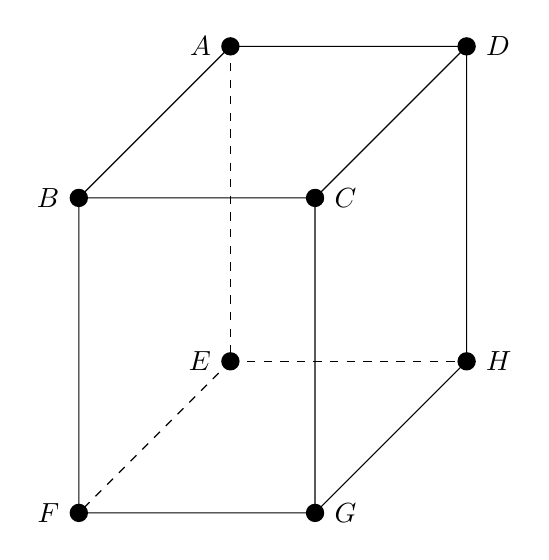
\begin{tikzpicture}[every edge quotes/.append style={auto, text=blue}]
				\pgfmathsetmacro{\cubex}{3}
				\pgfmathsetmacro{\cubey}{4}
				\pgfmathsetmacro{\cubez}{5}
				%%空間坐標中的CUBE 是以平面上的x軸 y軸再去擴充出深度z軸 z 往前為正,向後為負
				\coordinate (A) at (0,0,0);
				\coordinate (B) at (0,0,\cubez);
				\coordinate (C) at (\cubex, 0, \cubez );
				\coordinate (D) at (\cubex,0,0);
				\coordinate (E) at (0, -\cubey, 0);
				\coordinate (F) at (0, -\cubey, \cubez);
				\coordinate (G) at (\cubex, -\cubey, \cubez);
				\coordinate (H) at (\cubex, -\cubey, 0); 
				\draw [draw=black, every edge/.append style={draw=black, dashed}]
				(A) -- (B) --(C) --(D) -- cycle
				(C) -- (G) -- (H) -- (D) --cycle
				(B) -- (F) -- (G) -- (C) --cycle 
				(A) edge (E) 
				(E) edge (H)
				(E) edge (F);
				
				\foreach \v/\u/\t in 
				{A/180/$A$,
					B/180/$B$,
					C/0/$C$,
					D/0/$D$,
					E/180/$E$,
					F/180/$F$,
					G/0/$G$,
					H/0/$H$
				}
				{
					\draw[ultra thick,fill] (\v) circle (2.5pt);
					\node[label=\u:\t] at (\v){};
				};     
				\end{tikzpicture}
			\end{RightSidePic}
        \end{QBODY}
        \begin{QFROMS}
        \end{QFROMS}
        \begin{QTAGS}\QTAG{B4C1空間向量}\end{QTAGS}
        \begin{QANS}
            $\dfrac{4}{3}$
        \end{QANS}
        \begin{QSOLLIST}
			\begin{QSOL}
				\begin{LeftSide}[8cm]
					直角坐標坐標作法:\\
					\begin{QSTEPS}
						\QSTEP{ 令 $A(0,0,0), B(u,0,0), D(0,v,0), E(0,0,w) $}
						\QSTEP{ 由圖形可以知道平面$BDG$ 不會通過原點$A$,\\
							且與$x$, $y$, $z$ 軸皆有交點,且已知原平面過$B$, $D$ ,\\
							已有$x,y$ 截距,分別為 $u,v$\\
							可以假設 $E_{BDG}: \frac{x}{u} + \frac{y}{v} + \frac{z}{t} = 1$\\
							該平面通過$G(u,v,w)$ 代入可得:\\
							$1+1+\frac{w}{t}=1 \Rightarrow t= -w$\\
							$ \Rightarrow E_{BDG}: \frac{x}{u} + \frac{y}{v} + \frac{z}{-w} = 1 $
						}
						\QSTEP{ 由 $\lvec{AP} = \frac{1}{3} \lvec{AB} + 2 \lvec{AD} + a \lvec{AE} $\\
							可得點 $P$坐標為$ (\frac{1}{3} u, 2v, aw)$ \\
							且 $P$ 為平面 $BDG$ 上一點,\\
							代入滿足$E_{BDG}$ $\Rightarrow \frac{\frac{1}{3} u }{u}+\frac{2v}{v} + \frac{aw}{-w} = 1$ $\Rightarrow$\\
							 可解得 $a=\frac{4}{3}$ }
					\end{QSTEPS}
				\end{LeftSide}
				\begin{RightSidePic}
				   \begin{tikzpicture}
				   \pgfmathsetmacro{\cubex}{3}
				   \pgfmathsetmacro{\cubey}{4}
				   \pgfmathsetmacro{\cubez}{5}
				   %%空間坐標中的CUBE 是以平面上的x軸 y軸再去擴充出深度z軸 z 往前為正,向後為負
				   \coordinate (A) at (0,0,0);
				   \coordinate (B) at (0,0,\cubez);
				   
				   \coordinate (Bout) at (0,0,1.5*\cubez);
				   
				   \coordinate (C) at (\cubex, 0, \cubez );
				   \coordinate (D) at (\cubex,0,0);
				   
				   \coordinate (Dout) at (1.5*\cubex, 0, 0);
				   
				   \coordinate (E) at (0, -\cubey, 0);
				   
				   \coordinate (Eout) at (0, -\cubey *1.8, 0) ;
				   
				   \coordinate (F) at (0, -\cubey, \cubez);
				   \coordinate (G) at (\cubex, -\cubey, \cubez);
				   \coordinate (H) at (\cubex, -\cubey, 0); 
				   
				   \draw [draw=black, every edge/.append style={draw=black, dashed}]
				   (A) -- (B) --(C) --(D) -- cycle
				   (C) -- (G) -- (H) -- (D) --cycle
				   (B) -- (F) -- (G) -- (C) --cycle 
				   (A) edge (E) 
				   (E) edge (H)
				   (E) edge (F);
				   
				   \draw [fill=lightgray, opacity=0.5] (B)--(G)--(D) -- cycle;
				   
				   \draw[-{Stealth[scale=1.3,angle'=45]}, ultra thick] (A) -- (Dout) node[right] {$y$};
				   \draw[-{Stealth[scale=1.3,angle'=45]}, ultra thick] (A) -- (Bout) node[below] {$x$};
				   \draw[-{Stealth[scale=1.3,angle'=45]}, ultra thick] (A) -- (Eout) node[below] {$z$};
				   \foreach \v/\u/\t in 
				   {C/right/$C$,
					   F/left/$F$,
					   H/right/$H$
					}
					{
						\draw[ultra thick,fill] (\v) circle (2.5pt);
						\node[\u] at (\v){\t};
					};     
					\draw[ultra thick,fill] (A) circle (2.5pt);
					\draw[ultra thick,fill] (B) circle (2.5pt);
					\draw[ultra thick,fill] (D) circle (2.5pt);
					\draw[ultra thick,fill] (E) circle (2.5pt);
					\draw[ultra thick,fill] (G) circle (2.5pt);
					
					\node[above] at (A){$A(0,0,0)$};
					\node[label={[shift={(-1,0)}]$B(u,0,0)$} ] at (B) {};
					\node[above] at (D){$D(0,v,0)$};
					\node[right] at (G){$G(u,v,w)$};
					\node[label={[shift={(-1,0)}]$E(0,0,w)$}] at (E){};
					
					\end{tikzpicture}
				\end{RightSidePic}
			\end{QSOL}
        
			\begin{QSOL}
			   \begin{LeftSide}[8cm]
			   採用向量坐標\\

				   \begin{QSTEPS}
					   \QSTEP{令 $\lvec{AB}, \lvec{AD}, \lvec{AE}$ 為基底向量,$A$ 為坐標原點 \\
						   可知:$B(1,0,0),D(0,1,0), G(1,1,1) , P(\frac{1}{3}, 2 , a)$ }
						\QSTEP{先計算 $E_{BDG}:$\\
							找法向量:$\lvec{BD} = (-1,1,0), \lvec{BG} = (0,1,1) $\\
							$\Rightarrow \lvec{BD}\times \lvec{BG} = (1,1,-1) $ \\
							取法向量為 $\lvec{n} =(1,1,-1)$\\
							找點:$G(1,1,1)$ \\
							$\Rightarrow E_{BDG}: x+y-z=1$
						}
						\QSTEP{$P\in E_{BDG}$,$P$ 點坐標代入可得\\ $\frac{1}{3} + 2-a =1 \Rightarrow a = \frac{4}{3}$ }
					\end{QSTEPS}
				\end{LeftSide}
			   \begin{RightSidePic}
				   \begin{tikzpicture}
				   \pgfmathsetmacro{\cubex}{3}
				   \pgfmathsetmacro{\cubey}{4}
				   \pgfmathsetmacro{\cubez}{5}
				   %%空間坐標中的CUBE 是以平面上的x軸 y軸再去擴充出深度z軸 z 往前為正,向後為負
				   \coordinate (A) at (0,0,0);
				   \coordinate (B) at (0,0,\cubez);
				   
				   \coordinate (Bout) at (0,0,1.5*\cubez);
				   
				   \coordinate (C) at (\cubex, 0, \cubez );
				   \coordinate (D) at (\cubex,0,0);
				   
				   \coordinate (Dout) at (1.5*\cubex, 0, 0);
				   
				   \coordinate (E) at (0, -\cubey, 0);
				   
				   \coordinate (Eout) at (0, -\cubey *1.8, 0) ;
				   
				   \coordinate (F) at (0, -\cubey, \cubez);
				   \coordinate (G) at (\cubex, -\cubey, \cubez);
				   \coordinate (H) at (\cubex, -\cubey, 0); 
				   
				   \draw [draw=black, every edge/.append style={draw=black, dashed}]
				   (A) -- (B) --(C) --(D) -- cycle
				   (C) -- (G) -- (H) -- (D) --cycle
				   (B) -- (F) -- (G) -- (C) --cycle 
				   (A) edge (E) 
				   (E) edge (H)
				   (E) edge (F);
				   
				   \draw [fill=lightgray, opacity=0.5] (B)--(G)--(D) -- cycle;
				   
				   \draw[-{Stealth[scale=1.3,angle'=45]}, ultra thick] (A) -- (Dout) node[right] {$y$};
				   \draw[-{Stealth[scale=1.3,angle'=45]}, ultra thick] (A) -- (Bout) node[below] {$x$};
				   \draw[-{Stealth[scale=1.3,angle'=45]}, ultra thick] (A) -- (Eout) node[below] {$z$};
				   \foreach \v/\u/\t in 
				   {C/right/$C$,
					   F/left/$F$,
					   H/right/$H$
					}
					{
						\draw[ultra thick,fill] (\v) circle (2.5pt);
						\node[\u] at (\v){\t};
					};     
					\draw[ultra thick,fill] (A) circle (2.5pt);
					\draw[ultra thick,fill] (B) circle (2.5pt);
					\draw[ultra thick,fill] (D) circle (2.5pt);
					\draw[ultra thick,fill] (E) circle (2.5pt);
					\draw[ultra thick,fill] (G) circle (2.5pt);
					
					\node[above] at (A){$A(0,0,0)$};
					\node[label={[shift={(-1,0)}]$B(1,0,0)$} ] at (B) {};
					\node[above] at (D){$D(0,1,0)$};
					\node[right] at (G){$G(1,1,1)$};
					\node[label={[shift={(-1,0)}]$E(0,0,1)$}] at (E){};
					
					\end{tikzpicture}
				\end{RightSidePic}
			\end{QSOL}
        
		   \begin{QSOL}
			   採用共面定理:\\
			   $\lvec{AP} 
			   = \frac{1}{3}\lvec{AB} + 2 \lvec{AD} + a(\lvec{AG} - \lvec {AB} -\lvec{AD} ) 
			   = (\frac{1}{3} - a) \lvec{AB} + (2-a) \lvec{AD} + a \lvec{AG} $
			   
			   根據共面定理可得:$(\frac{1}{3} - a) + (2-a) +a = 1 \Rightarrow a = \frac{4}{3} $\\
			   \vspace{1.5cm}\\
			   \psset{cornersize=absolute,linearc=.2\baselineskip} 
			   \psframebox[framesep=15pt]
			   {		
				   \begin{minipage}[c]{14cm}
					   共面定理:在空間坐標中,$O$ 與 $A,B,C$ 不共面, 有一點 $P$ \\
					   使得 $\lvec{OP} = \alpha \lvec{OA} +\beta \lvec{OB} +\gamma \lvec{OC} $ \\
					   若 $A,B,C,P$ 共面 ,則$\alpha+\beta+\gamma = 1$
					\end{minipage}
				}
			\end{QSOL}
        \end{QSOLLIST}
        \begin{QEMPTYSPACE}
        \end{QEMPTYSPACE}
    \end{QUESTION}
\end{QUESTIONS}
